%%% The main file. It contains definitions of basic parameters and includes all other parts.

%% Settings for single-side (simplex) printing
% Margins: left 40mm, right 25mm, top and bottom 25mm
% (but beware, LaTeX adds 1in implicitly)
\documentclass[12pt,a4paper,rgb]{report}
\setlength\textwidth{145mm}
\setlength\textheight{247mm}
\setlength\oddsidemargin{15mm}
\setlength\evensidemargin{15mm}
\setlength\topmargin{0mm}
\setlength\headsep{0mm}
\setlength\headheight{0mm}

% \openright makes the following text appear on a right-hand page
\let\openright=\clearpage

%% Settings for two-sided (duplex) printing
% \documentclass[12pt,a4paper,twoside,openright]{report}
% \setlength\textwidth{145mm}
% \setlength\textheight{247mm}
% \setlength\oddsidemargin{14.2mm}
% \setlength\evensidemargin{0mm}
% \setlength\topmargin{0mm}
% \setlength\headsep{0mm}
% \setlength\headheight{0mm}
% \let\openright=\cleardoublepage

%% Generate PDF/A-2u
\usepackage[a-2u]{pdfx}

%% Character encoding: usually latin2, cp1250 or utf8:
\usepackage[utf8]{inputenc}
\usepackage[T1]{fontenc}	% ľľľ in abstract

%% Prefer Latin Modern fonts
\usepackage{lmodern}

%% Further useful packages (included in most LaTeX distributions)
\usepackage{amsmath}        % extensions for typesetting of math
\usepackage{amsfonts}       % math fonts
\usepackage{amsthm}         % theorems, definitions, etc.
\usepackage{bbding}         % various symbols (squares, asterisks, scissors, ...)
\usepackage{bm}             % boldface symbols (\bm)
\usepackage{graphicx}       % embedding of pictures
\usepackage{fancyvrb}       % improved verbatim environment
\usepackage{natbib}         % citation style AUTHOR (YEAR), or AUTHOR [NUMBER]
\usepackage[nottoc]{tocbibind} % makes sure that bibliography and the lists
			    % of figures/tables are included in the table
			    % of contents
\usepackage{dcolumn}        % improved alignment of table columns
\usepackage{booktabs}       % improved horizontal lines in tables
\usepackage{paralist}       % improved enumerate and itemize
\usepackage{xcolor}         % typesetting in color
\usepackage{enumitem}		% enumerations with letters, etc
\usepackage{tikz}			% Graphs
\usetikzlibrary{patterns}

\usepackage{listings}		% Listings 
\usepackage{adjustbox}

%%% Basic information on the thesis

% Thesis title in English (exactly as in the formal assignment)
\def\ThesisTitle{A programming language presented in graphics}
\def\ThesisTitleSK{Graficky prezentovaný programovací jazyk}

% Author of the thesis
\def\ThesisAuthor{Roman Sobkuliak}

% Year when the thesis is submitted
\def\YearSubmitted{2020}

% Name of the department or institute, where the work was officially assigned
% (according to the Organizational Structure of MFF UK in English,
% or a full name of a department outside MFF)
\def\Department{Department of Software Engineering}
\def\DepartmentSK{Katedra softwarového inžinierstva}

% Is it a department (katedra), or an institute (ústav)?
\def\DeptType{Department}
\def\DeptTypeSK{Katedra}

% Thesis supervisor: name, surname and titles
\def\Supervisor{RNDr. David Bednárek, Ph.D.}

% Supervisor's department (again according to Organizational structure of MFF)
\def\SupervisorsDepartment{Department of Software Engineering}
\def\SupervisorsDepartmentSK{Katedra softwarového inžinierstva}

% Study programme and specialization
\def\StudyProgramme{Computer Science}
\def\StudyBranch{Software and Data Engineering}

% An optional dedication: you can thank whomever you wish (your supervisor,
% consultant, a person who lent the software, etc.)
\def\Dedication{%
I would like to give thanks to my supervisor, RNDr. David Bednárek, Ph.D., for his time
and advice, and also to my parents for their extensive support and patience.
}

% Abstract (recommended length around 80-200 words; this is not a copy of your thesis assignment!)
\def\Abstract{%
The goal of this thesis is to create a programming language with characters and keywords substituted
with images and animations (GIFs). We build a web IDE and a client-side interpreter for this language
using modern web technologies including WebWorkers, TypeScript and React.

The IDE features a code-stepping with information about current location in the source
code, environment variables and a call stack. Additionally, there is a support for storing programs on the server
and loading them later.

Primarily, it will be used at programming camps for elementary and high schoolers. The author of this thesis designs
creative games for these camps, usually related to Computer Science. The language created in this thesis will
be incorporated into the games.

At the time of writing, we could not find any other such programming language.
}

\def\AbstractSK{%
Cieľom práce je vytvoriť programovací jazyk so znakmi a kľúčovými slovami nahradenými za obrázky a animácie (GIFy).
To zahŕňa naprogramovanie webového vývojového prostredia a interpreteru pre tento jazyk.
V práci využijeme moderné webové technológie ako WebWorkers, TypeScript a React.

Vývojové prostredie podporuje krokovanie programu s informáciami o aktuálnej pozícii v kóde, hodnotami premenných a
volacieho zásobníku. Vývojové prostre\-die navyše ponúka možnosť ukladať a načítať užívateľské programy zo serveru.

Primárne bude tento jazyk použitý na základoškolských a stredoškolských programovacích sústredeniach. Autor práce
tvorí kreatívne táborové hry pre tieto sústredenia, typicky spojené s programovaním. Jazyk vytvorený v tejto práci
bude zahrnutý v týchto hrách.

V čase písania práce sa nám nepodarilo nájsť jazyk podobný tomu, ktorý tvoríme v tejto práci.
}

% 3 to 5 keywords (recommended), each enclosed in curly braces
\def\Keywords{
{Visual programming language} {Program interpretation} {Code-stepping} {GIF language}
}
\def\KeywordsSK{
{Vizuálny programovací jazyk} {Interpreter programu} {Krokovanie kódu} {GIFový jazyk}
}

%% The hyperref package for clickable links in PDF and also for storing
%% metadata to PDF (including the table of contents).
%% Most settings are pre-set by the pdfx package.
\hypersetup{unicode}
\hypersetup{breaklinks=true}

% Definitions of macros (see description inside)
\include{macros}

% Title page and various mandatory informational pages
\begin{document}
\include{title}

%%% A page with automatically generated table of contents of the bachelor thesis

\tableofcontents

%%% Each chapter is kept in a separate file
\chapter{Introduction}

Typical programming languages are defined in terms of plaintext tokens. These tokens
are then used in grammar rules to specify which orderings of tokens are valid programs and
which are not.
\begin{figure}[!hbt]
	\includegraphics[width=\textwidth]{../img/tokens_and_grammar}
	\caption{Sample language definition with examples}
	\label{fig:chap1:tokens_and_grammar}
\end{figure}

On the figure \ref{fig:chap1:tokens_and_grammar} we see a set of token rules and grammar rules defining a~simple
language. Sample program $1$ shows a valid program in this language with its respective derivation tree, while
second program does not adhere to the defined grammar rules.
While given example is trivial it shows how vast majority of programming languages are defined and processed:
\begin{itemize}
\item Users write plaintext source code
\item Lexical analysis splits the source code into tokens based on the rules provided
\item Syntax analysis builds a tree (AST or derivation tree) based on the grammar rules
\item AST is used to compile, interpret or transpile the source code
\end{itemize}

However, tokens do not have to consist of plaintext necessarily. Plaintext characters can be substituted for
images, videos, sounds, etc. In this thesis we construct a programming language with characters and some
of the tokens substituted for images or short looping videos (e.g. GIFs). A Figure \ref{fig:chap1:giflang_code} below shows
the Sample program 1 from \ref{fig:chap1:tokens_and_grammar} written in Giflang\footnote{We named the programming
language developed in this thesis Giflang}.
\begin{figure}[!hbt]
	\includegraphics[width=\textwidth]{../img/giflang_code}
	\caption{Sample code in Giflang}
	\label{fig:chap1:giflang_code}
\end{figure}

You can see that characters and digits have their counterparts in Giflang. Assignment is represented with an arrow,
thumbs up is a semicolon and `print' function is a single image containing paper. The exact choice of images used here is of course
not very relevant.

In order to be able to store and parse programs like that we also need to define an intermediate
format. The format can be for example textual and the sample program from Figure \ref{fig:chap1:giflang_code} can be written as:
\begin{code}
Z;E;R;O; ASSIGN; 0; SEMICOLON;
PRINT; LPAR; Z;E;R;O; RPAR; SEMICOLON;
\end{code}

We actually chose the format shown above. We discuss the intermediate format and the language design in section /TODO/.

You can see that there is a clear mapping between images and semicolon-delimited tokens. Therefore, a byproduct of
this thesis is a token-level programming language, i.e. a language that consists of delimited tokens. This tokens
can have different presentational forms as mentioned before.

A language like this one is of course impractical and hard to follow. We do not intend to create a language
for practical use. Our $3$ main motivations for creating Giflang are:
\begin{enumerate}
\item An image-based programming language like this does not exist yet. We discuss other existing visually oriented
languages in section /TODO/. 
\item Using it in bootcamps for elementary and high schoolers. We co-organize a long-term Computer Science competition
named Prask\footnote{prask.ksp.sk todo}. After each semester we invite best contestants to a week-long bootcamp
filled with creative games mostly related to Computer Science. Giflang can be used as part of the games.
\item Allowing users to substitute images for their own can give younger users feeling of creating ''their own language''.
\end{enumerate}

Since we use images instead of characters we need to implement our own IDE to be able to create and run Giflang programs. Typically,
IDEs are desktop applications. However, since ease of access and use have bigger priority than efficiency for this application
we decided to move everything to a browser.

To sum up it up, in this thesis we design a programming language with characters and some of the tokens substituted for images.
Additionally, we build an interpreter and an IDE for this language that both run in browser. Goals mentioned here are described
more precisely in the Section \ref{chap1:thesis_goals}. 

\section{Related work}
\cite{Andel07}
Visual programming languages have been around since ... and this thesis was undeniably inspired by them. A visual 
programming language lets users create programs by manipulating program elements graphically rather than by specifying them textually\footnote{Wikipedia}.
Giflang is not a visual programming language as users can not manipulate with graphics in its IDE, e.g. move it, connect it with other
objects, etc. It is also not a textual language per-se as text is replaced by images. However, it is definitely closer to a textual
rather than a visual programming language so we could say that it is a semi-textual programming language.

This section will discuss programming languages we got inspired from and also multiple web IDEs since we implement
Giflang for web.

\subsection{Emojicode}
An excerpt from the official documentation: Emojicode is an open source, high-level, multi-paradigm programming language consisting of emojis.
It features Object-Orientation, Optionals, Generics and Closures.

Here is a `Hello World' program in Emojicode:
\begin{figure}[!hbt]
	\includegraphics[width=0.5\textwidth]{../img/emojicode_helloworld}
	\label{fig:chap1:emojicode_helloworld}
\end{figure}

All built-in keywords and most of the special characters are replaced by emojis. For example a raspberry is an opening curly brace `{' in Emojicode.
However, as you can on the `Hello World' program not every character is replaced by an emoji. Additionally, users can not create their own emoji
mappings to keywords or characters. Creating Emojicode sources is simple as emojis are just Unicode characters and most of the modern text editors
have a good support for them.

For compilation Emojicode uses LLVM which is a collection of reusable compiler technologies. Source code is compiled first to LLVM IR\footnote{IR or
Intermediate Language is a low-level programming language similar to assembly.} and then to machine code. With features as compilation to an intermediate
language, object-orientation, static typing and garbage collection we can say Emojicode is similar to languages like C\# or Java.

Emojicode is the closest language to the one we build in this thesis. However, since we are replacing characters and keywords with arbitrary images as
opposed to emojis we have to use an intermediate textual format that maps to the images. Emojicode does not have this problem since emojis are
Unicode characters that can be represented in plaintext and parsed.

\subsection{Karel?}
\subsection{REPl?}

\section{IDE as desktop vs browser application}

\section{Thesis goals}
\label{chap1:thesis_goals}
\chapter{Language design}

\section{Reusing an existing language vs creating a new one}

\section{Deciding on language type}
OOP vs functional vs esoteric vs ...

\section{Source code representation}
tokens delimited with semicolons

\chapter{Language design}
\label{chap3:language_design}

When creating Giflang we had two options:
\begin{enumerate}
    \item Use a~language with an~existing web interpreter
    \item Create a~new language and a~web interpreter
\end{enumerate}

In~the~first section of this chapter we explain~why we decided to not reuse an~existing language. In this section we discuss the~design of our own language. We do not
precisely define all the~semantics, but rather provide a~high-level overview. We think that it is more important to explain~\emph{why} Giflang uses specific
constructs, rather than~list \emph{how} these constructs behave in~every case.

The~language documentation with examples can~be found in~the~web IDE by clicking ``Docs'' button in the top navigation.

\section{Reusing an~existing interpreter}
in~the~previous Chapter \ref{chap2} we concluded that interpreting a~user code on the~client-side is the~best option for our project. Therefore, when
looking for a~language to reuse we need to limit ourselves to the~ones that have an~existing web interpreter, i.e., an~interpreter written in~either
JavaScript or WebAssembly. The~two major languages that have existing web interpreters are Python and JavaScript.

\subsection{Python}
There are multiple Python web interpreters, for example Pyodide \cite{Pyodide} or Brython \cite{Brython}. Pyodide works by compiling CPython \cite{CPython}
to WebAssembly using Emscripten. Brython works by transpiling Python to JavaScript. We were not able to find a~Python web interpreter that would
support code-stepping out of the~box. We considered forking either Pyodide or Brython and adding this functionality.

Adding code-stepping to Pyodide would require changing the~underlying CPy\-thon implementation. CPython is very complex and was not built for this use case.
On the~other hand, Brython is fully written in~JavaScript and also builds an~AST from a~Python code in~JavaScript. There
is even a~fork of Brython \cite{PythonDebugger} that implements code-stepping. However, at closer inspection we found out it runs the~code all at once and records trace information
at each executed line by inserting a~trace function call there. Afterwards, it only gives users an~illusion of code-stepping.

It is possible to create a~``live'' code-stepping for Brython in~a~similar fashion, for example with the~aid of Atomics API discussed in~Section \ref{chap4:atomics}.
We did not find a~simple way of increasing the~stepping granularity from just lines to arbitrary AST nodes, though. We definitely could have adjusted Brython instead
of creating a~custom interpreter. However, it would take a~non-trivial effort to change the~Brython's internals and we rather put this effort into creating
a~new interpreter from scratch and learning a~lot about languages and interpreters along the~way. Additionally, we did not have a lot of experience with writing
interpreters and compilers prior to this project and hence it would be quite challenging to customize an existing one.

\subsection{JavaScript}
\label{chap3:javascript}
There are numerous JavaScript interpreters written in~JavaScript. The~one closest to our needs is JS-Interpreter \cite{JSInterpreter} that supports running JavaScript
with code-stepping in~isolation. It was designed for use in~Blockly \cite{Blockly}, a~library for building visual programming editors.

JS-Interpreter supports only ES5\footnote{ECMAScript 5 or ECMAScript 2009} standard of JavaScript. This standard has no \texttt{class} keyword or block-scoped
variables with \texttt{let} keyword. We find ES5 way of defining classes using functions and prototypes confusing:
\begin{code}
// ES 5
function Person(name) {
    this.name = name;  
}

Person.prototype.greet = function () {
    console.log('Hello my name is ' + this.name);
}

// ES 6
class Person {
    constructor(name) {
        this.name = name
    }

    greet() {
        console.log('Hello my name is ' + this.name);
    }
}
\end{code}

We could add support for ES6 features to the~JS-Interpreter and use it for our project. However, as in~the~case of Brython we decided to rather put the~effort into
creating a~new solution than~putting a~lot of effort an~existing one.

\section{Text format}
Before we dive into the~language itself, let us first discuss the~underlying representation of the~language. We could represent programs either
in a \emph{binary format} or a \emph{textual format}. Using a binary format, we could map images to numbers and considering that our ``alphabet of images''
would be at most 256 characters long, we could use one byte per image. However, it is much simpler to develop the language with a textual format because
when writing tests and debugging we can work with printable characters rather than seemingly random numbers. Therefore, we decided to use a textual format.

We considered defining the~language in~terms of semicolon delimited tokens where each token could be substituted with a~single image.
Below is an~identity function defined in~both a~\emph{token-level} and a~\emph{character-level format}.
\begin{code}
// Token-level
FUNCTION; I;D; LPAR; A; RPAR; LCURLY;
RETURN; A; SEMICOLON;
RCURLY;

I;D; LPAR; 8; RPAR; SEMICOLON;

// Character-level
function ID(A) {
    return A;
}

ID(8);
\end{code}

A simpler option is to represent keywords as single characters in~the~character-level format. This makes the~image substitution trivial, as we can~substitute
every character. The~``keyword characters'' have to be unique among other characters. To illustrate this, we can~use a~Unicode letter `f' with a~hook $f$
to represent a~function and a~character $\hookleftarrow$ for return.
\begin{code}
$f$ ID(A) {
    $\hookleftarrow$ A;
}

ID(8);
\end{code}

The~above approach that uses Unicode characters has a~nice property regarding the~use of the~keywords in~a~string. According to the~ECMAScript specification,
Section 8.4 \cite{Ecmascript}: \emph{When a~String contains actual textual data, each element is considered to be a~single UTF-16 code unit.} This means that if we
only use characters that can~be encoded into a~single 16-bit code unit, all keywords will take space of a~single character in~a~string.

At first we used the~token-level format. It made the~implementation of the~parser harder because typical lexer responsibilities like processing
an~identifier had to be moved to the~syntactical analysis. Later on, we decided to switch to the~character-level format with keywords substituted for
Unicode characters. We changed the~format mostly because we realized that the~token-level format only introduced more complexity with no real benefits.

\section{Deciding on a~language type}
Since we have chosen to build our own language it is time to decide on what kind of language it should be and what features it should have. There are
multiple types of programming languages and we will briefly go through the~most known ones.

\subsection{Functional programming}
Functional programming treats computation as an~evaluation of mathematical functions and avoids changing state and mutable
data.\footnote{https://en.wikipedia.org/wiki/Functional\_programming}
This means that functional programming languages do not support imperative flow controls like loop statements.

Pure functions are very typical for functional programming. \emph{Pure functions} are functions whose outcome depends solely on their arguments
and create no side-effects (e.g., by changing a~global variable). Eliminating side effects can~make understanding a~program easier, which is one of the
key motivations for the~development of functional programming.

Additionally, functional programming often relies on recursion and functions being first-class entities. Being a~first-class entity means that functions can~appear
anywhere in~the~program where other first-class entities like numbers can, including arguments to other functions and their return values.

One of the~typical examples of a~functional programming language is Haskell. It was created in~1990, it is statically typed, supports type inference,
and lazy evaluation. Below is a~sample program in~Haskell finding the~edit distance between two strings from the~official docs.
\begin{code}
import Data.Array as Array

editDistance :: Eq a~=> [a] -> [a] -> Int
editDistance xs ys = table ! (m,n)
    where
    (m,n) = (length xs, length ys)
    x     = array (1,m) (zip [1..] xs)
    y     = array (1,n) (zip [1..] ys)
    
    table :: Array (Int,Int) Int
    table = array bnds [(ij, dist ij) | ij <- range bnds]
    bnds  = ((0,0),(m,n))
    
    dist (0,j) = j
    dist (i,0) = i
    dist (i,j) = minimum [table ! (i-1,j) + 1, table ! (i,j-1) + 1,
        if x ! i == y ! j
            then table ! (i-1,j-1)
            else 1 + table ! (i-1,j-1)]
\end{code}

\subsection{Object-oriented programing}
Object-oriented programming (OOP) is based around the~concept of ``objects'' which can~contain~data, in~the~form of fields (also known as attributes or properties),
and code, in~the~form of methods.\footnote{https://en.wikipedia.org/wiki/Object-oriented\_programming} Object's methods can~access and modify the~object they are
operating on using a~keyword like \texttt{this} or \texttt{self}. Programs then made out of objects that interact together.

The~most popular OOP languages are class-based (e.g., C++, Java, Python), meaning that objects are instances of classes, which also determine their types.
There are also alternatives, for example JavaScript is prototype-based.

OOP has a~few features that are common among most of the~object-oriented programming languages:
\begin{itemize}
    \item Inheritance or subclassing lets developers create a~new class by building upon an~existing one.
    \item Encapsulation allows hiding data~and methods of an~object from the~outside interference and misuse.
    \item Polymorphism allows calling code to be agnostic as to which class in~the~supported hierarchy it is operating on.
\end{itemize}

Below is an~example of polymorphism in~C++.
\begin{code}
class Animal {
public:
    virtual ~Base() { }
    virtual string make_sound() = 0;
};

class Dog: public Animal {
public:
    string make_sound() { 
        return "Woof, woof!"; 
    }
};

class Sheep: public Animal {
public:
    string make_sound() { 
        return "Baa, baa!"; 
    }
};

int main() {
    Animal *animal;
    Dog dog;
    Sheep sheep;

    // Store the~address of Dog.
    animal = &dog;

    // Call Dog's make_sound. Returns "Woof, woof!".
    animal->make_sound();
    // A~similar example with sheep. Returns "Baa, baa!".
    animal = &sheep;
    animal->make_sound();

    return 0;
}
\end{code}

\subsection{Esoteric programming languages}
An~esoteric programming language is designed to experiment with weird ideas, to be hard to program in, or as a~joke, rather than~for practical use. We can~not
describe esoteric languages in~general as they all use different ideas.

Probably the~most popular esoteric language is brainf***. It operates on an~array of memory cells, also referred to as the~tape. All of the~cells are initially
set to zero. There is a~single pointer, initially pointing to the~first memory cell. The~language has the~following commands:

\begin{figure}[!hbt]
    \centering
    \begin{tabular}{|c l |} 
    \hline
    $>$ & Move the~pointer to the~right \\
    \hline
    $<$ & Move the~pointer to the~left \\
    \hline
    $+$ & Increment the~memory cell under the~pointer \\
    \hline
    $-$ & Decrement the~memory cell under the~pointer \\
    \hline
    $.$ & Output the~character signified by the~cell at the~pointer \\
    \hline
    $,$ & Input a~character and store it in~the~cell at the~pointer \\
    \hline
    $[$ & Jump past the~matching ] if the~cell under the~pointer is 0 \\
    \hline
    $]$ & Jump back to the~matching [ if the~cell under the~pointer is nonzero \\
    \hline
    \end{tabular}
    \caption{a~list of brainf*** commands}
\end{figure}

Other examples of esoteric languages are:
\begin{itemize}
    \item Shakespeare, a~programming language whose source code resembles Shakespeare plays. 
    \item Befunge, a~language where the~code is layed out on a~two-dimensional grid of instructions, and execution can~proceed in~any direction of that grid.
\end{itemize}

\subsection{Conclusion}
There are also other programming language types apart from the~ones mentioned here, for example logic programming. We did not plan~on using
concepts from these languages and hence we did not list them. It would be great to combine a~language presented in~images with an~esoteric language
of some sort. However, we did not come up with an~interesting enough model and we did not want to blindly reuse an~existing one. in~the~end we settled on
a~more conservative approach.

Since our intended audience is typically experienced in~Python we decided to base our language around "Pythonic" features. We also think
the~class-based model of Python is more intuitive than~prototype-based one found for example in~JavaScript.

Even though the~author of this thesis likes statically-typed languages, Giflang is dynamically-typed. The~primary reason is that images take a~lot of
space on the~user screen and hence we tried to keep the~language concise. Adding typed declarations would probably make it less error-prone, but more verbose.

\section{Object model}
\label{chap3:object_model}
As mentioned in~the~end of the~previous section we base Giflang on Python. Everything is an~object in~Python. We will now explain~in~more detail what exactly
it means. an~object \texttt{A} can~have multiple related objects:
\begin{itemize}
    \item An~object \texttt{B} that denotes the~type of \texttt{A}. We call \texttt{B} a~\emph{class}\footnote{In the implementation we denote this \texttt{klass}
    instead of \texttt{class} because of a name collision with the keyword \texttt{class}.} of the~instance \texttt{A} and we say that \texttt{A}
    is an~instance of \texttt{B}.
    \item If \texttt{A} is a~class it can~have multiple \emph{base classes}. Let \texttt{B} denote one of the~base classes. We say that \texttt{A}
    \emph{derives from} \texttt{B}. 
\end{itemize}

Since classes are objects, they have to be instances of \emph{some} class. We call this ``class of classes'' a~\texttt{MetaClass}. Of course
\texttt{MetaClass} is also an~object and thus has to be an~instance of \emph{some} class. To break the~chain, \texttt{MetaClass} is an~instance of itself.
Figure \ref{fig:chap3:python_structure} describes the~Python's object structure in~more detail.

\begin{figure}[!hbt]
    \centering
    \tikzset{every picture/.style={line width=0.75pt}} %set default line width to 0.75pt        
    \trimbox{0cm .75cm 0cm 0cm}{
        \begin{tikzpicture}[x=0.75pt,y=0.75pt,yscale=-1,xscale=1]
        \draw   (13.61,159.25) -- (125.73,159.25) -- (125.73,200.19) -- (13.61,200.19) -- cycle ;
        \draw    (67.11,199.26) .. controls (87.27,268.92) and (-12.63,252.81) .. (12.38,202.52) ;
        \draw [shift={(13.61,200.19)}, rotate = 479.36] [fill={rgb, 255:red, 0; green, 0; blue, 0 }  ][line width=0.08]  [draw opacity=0] (10.72,-5.15) -- (0,0) -- (10.72,5.15) -- (7.12,0) -- cycle    ;
        \draw   (14.54,80.16) -- (126.66,80.16) -- (126.66,121.1) -- (14.54,121.1) -- cycle ;
        \draw  [dash pattern={on 0.84pt off 2.51pt}]  (58.73,160.18) -- (58.73,129.48) -- (58.73,125.03) ;
        \draw [shift={(58.73,122.03)}, rotate = 450] [fill={rgb, 255:red, 0; green, 0; blue, 0 }  ][line width=0.08]  [draw opacity=0] (10.72,-5.15) -- (0,0) -- (10.72,5.15) -- (7.12,0) -- cycle    ;
        \draw    (82,122.03) -- (82,155.32) ;
        \draw [shift={(82,158.32)}, rotate = 270] [fill={rgb, 255:red, 0; green, 0; blue, 0 }  ][line width=0.08]  [draw opacity=0] (10.72,-5.15) -- (0,0) -- (10.72,5.15) -- (7.12,0) -- cycle    ;
        \draw   (163.41,159.25) -- (275.54,159.25) -- (275.54,200.19) -- (163.41,200.19) -- cycle ;
        \draw    (162.95,179.72) -- (129.66,179.72) ;
        \draw [shift={(126.66,179.72)}, rotate = 360] [fill={rgb, 255:red, 0; green, 0; blue, 0 }  ][line width=0.08]  [draw opacity=0] (10.72,-5.15) -- (0,0) -- (10.72,5.15) -- (7.12,0) -- cycle    ;
        \draw  [dash pattern={on 0.84pt off 2.51pt}]  (216.45,159.25) -- (130.12,104.11) ;
        \draw [shift={(127.59,102.49)}, rotate = 392.57] [fill={rgb, 255:red, 0; green, 0; blue, 0 }  ][line width=0.08]  [draw opacity=0] (10.72,-5.15) -- (0,0) -- (10.72,5.15) -- (7.12,0) -- cycle    ;
        \draw   (313.22,149.02) -- (425.35,149.02) -- (425.35,209.5) -- (313.22,209.5) -- cycle ;
        \draw    (312.76,179.72) -- (279.47,179.72) ;
        \draw [shift={(276.47,179.72)}, rotate = 360] [fill={rgb, 255:red, 0; green, 0; blue, 0 }  ][line width=0.08]  [draw opacity=0] (10.72,-5.15) -- (0,0) -- (10.72,5.15) -- (7.12,0) -- cycle    ;
        \draw    (286.5,76.74) -- (223.15,76.74) ;
        \draw [shift={(220.15,76.74)}, rotate = 360] [fill={rgb, 255:red, 0; green, 0; blue, 0 }  ][line width=0.08]  [draw opacity=0] (10.72,-5.15) -- (0,0) -- (10.72,5.15) -- (7.12,0) -- cycle    ;
        \draw  [dash pattern={on 0.84pt off 2.51pt}]  (286.5,110.74) -- (223.15,110.74) ;
        \draw [shift={(220.15,110.74)}, rotate = 360] [fill={rgb, 255:red, 0; green, 0; blue, 0 }  ][line width=0.08]  [draw opacity=0] (10.72,-5.15) -- (0,0) -- (10.72,5.15) -- (7.12,0) -- cycle    ;
        \draw (69.67,179.72) node   [align=left] {{\fontfamily{pcr}\selectfont MetaClass}};
        \draw (70.6,100.63) node   [align=left] {{\fontfamily{pcr}\selectfont ObjectClass}};
        \draw (219.48,179.72) node   [align=left] {{\fontfamily{pcr}\selectfont UserClass}};
        \draw (370.87,179.72) node   [align=left] {{\fontfamily{pcr}\selectfont  UserClass}\\{\fontfamily{pcr}\selectfont instance}};
        \draw (351.87,75.72) node   [align=left] {{\fontfamily{pcr}\selectfont Instance of}};
        \draw (357.87,110.72) node   [align=left] {{\fontfamily{pcr}\selectfont Derives from}};
        \end{tikzpicture}
    }
    \caption{Object structure in~Python.}
	\label{fig:chap3:python_structure}
\end{figure}

\texttt{MetaClass} is actually called \texttt{type} in~Python. Below is an~interactive Python session that unveils the~internals of Python shown
in~Figure \ref{fig:chap3:python_structure}.
\begin{code}
>>> class X:
...     pass
... 
>>> type(X)
<class 'type'>
>>> x = X()
>>> type(x)
<class '__main__.X'>
>>> type(type(X))
<class 'type'>
>>> type(X).__bases__
(<class 'object'>,)
>>> type(type(X).__bases__[0])
<class 'type'>
\end{code}

We decided to reuse this model as the~base of Giflang. To make things simple we decided to not support multiple inheritance, though.

\subsection{Magic Methods}
Another Python feature we reused are magic methods. They provide a~very straightforward way
to overload operators. Magic methods are prefixed and suffixed with two underscores. Below is a~Python example that uses magic methods:
\begin{code}
class Number:
    # Defines a~constructor
    def __init__(self, val):
        self.val = val
    
    # Defines a~string representation
    def __str__(self):
        return str(self.val)

    # Overloads operator +
    def __add__(self, other):
        return Number(self.val + other.val)

    # Overloads a~call operator
    def __call__(self):
        return 'an~instance was called :)'

x = Number(2)
y = Number(3)
# Outputs 5. First __add__ is called and then __str__ on the~result.
print(x + y)
# Outputs 'an~instance was called :)'
print(x())
\end{code}

The~example shows how to create a~constructor, overload an~operator and create a~new instance of a~class by calling the~class with arguments for the~constructor.
\texttt{Number} class also defines a~\texttt{\_\_call\_\_} method so naturally we might expect the~call \texttt{Number(2)} to result in~the~string
`an~instance was called :)'. However, it is not the~case. Instead, \texttt{Number(2)} results in~a~new instance of the~\texttt{Number} class. The~author of this
thesis thinks that this is the~reason why magic method resolution in~Python starts from the~instance type rather than~from the~instance itself, as it is
the~case with regular methods.

Because the~call \texttt{Number(2)} does not result in~the~call of the~\texttt{\_\_call\_\_} function on the
\texttt{Number} type, it has to result in~a~\texttt{\_\_call\_\_} method further up the~chain. in~this case, \texttt{Number} is an~instance of the~\texttt{type},
or the~\texttt{MetaClass} class. Its \texttt{\_\_call\_\_} method is responsible for creating a~new instance and calling the~\texttt{\_\_init\_\_} method. Oversimplified,
the~\texttt{type}'s \texttt{\_\_call\_\_} function might look like this:
\begin{code}
class type:
    # Since classes are instances of the~'type' class, self
    # in~this method is a~class object. 
    def __call__(self, *args, **kwargs):
        obj = instantiate(self)
        obj.__init__(*args, **kwargs)
        return obj
\end{code}

in~reality, creating a~new instance is a~little more complicated. To give users more control over the~instantiation, another magic method (\texttt{\_\_new\_\_})
is called instead of a~made up function \texttt{instantiate} in~the~example above. We will not go into more details since we decided not to include the
\texttt{\_\_new\_\_} magic method into Giflang as it is mainly used only for a~few specific use cases (e.g., creating a~singleton).

Having a~keyword for introducing new variables, e.g., \texttt{var}, would mean~that magic methods could be resolved the~same way as normal methods because
it would allow us to distinguish between instantiation calls, e.g., \texttt{Number(3)}, and regular method call. However,
we like the~simplicity of creating a~new instance via~calling a~class and hence used this approach in~Giflang as well.

\section{Basic types}
There are 7 basic types supported natively in~Giflang: \texttt{Object}, \texttt{Number}, \texttt{Boolean}, \texttt{None}, \texttt{Function},
\texttt{Array} and \texttt{String}.

Since the~interpreter is written in~JavaScript, we based the~types mostly around JavaScript types; for example \texttt{Number} is a~wrapper of the~JavaScript
\texttt{number}. Because of this, it has a~standard double-precision 64-bit floating point format (IEEE 754). Booleans \texttt{True} and \texttt{False}
and also \texttt{None} are all represented using a~single image. in~the~language itself they are just global variables, similar to Python.

Functions are first-class entities, which means that users can~create anonymous functions, pass callbacks, etc. Closures are also supported.
Arrays and strings are basically wrappers around JavaScript arrays and strings as it was the~simplest approach. There are no primitive types and everything is
an~\texttt{Object}. Of course, it would be more effective to implement the~\texttt{Number} as a~primitive type, but as stated earlier, performance was not one
of the~main~objectives and implementing the~\texttt{Number} as an~\texttt{Object} was easier.

As with any other language, there needs to be a~support for basic conversions. We could create explicit conversion functions, but since Giflang is dynamically typed,
we implemented conversions in~the~constructors of the~target types. For example, calling \texttt{Number('1')} should result in~a~conversion from a~\texttt{String} to
a~\texttt{Number}.

\section{Control flow constructs}
Giflang supports the~following control flow constructs: \texttt{if}, \texttt{while} and \texttt{for}. The author of this thesis is a~fan~of the~C-like \texttt{for}
and thus used it in~Giflang as well. When evaluating a~condition, a~\texttt{\_\_bool\_\_} magic method is called on the~resulting object to convert it to
a~\texttt{boolean}. By default, everything except for \texttt{0}, \texttt{None}, \texttt{False}, an~empty string and an~empty array, evaluates to \texttt{True}.

\section{Standard library}
Giflang's standard library is quite modest. There is only support for the~very basics: \texttt{array}, \texttt{string}, \texttt{I/O}. As mentioned earlier, arrays
and strings wrap standard JavaScript arrays and strings. The~I/O is provided in~the~form of three functions:
\begin{itemize}
    \item \texttt{input} function reads a~single line
    \item \texttt{println} calls \texttt{\_\_str\_\_} magic method on its arguments to stringify them and outputs them on a~single line, space separated and
    with a~newline at the~end
    \item \texttt{print} has the~same semantics as \texttt{println}, but omits the~newline at the~end
\end{itemize}

We did not extend the~library further since arrays, strings and I/O are the~necessary building blocks that should suffice for most of the~basic use-cases.
Extending the~library further would not be hard, but we decided to invest the~time into different areas of the~project.
\chapter{Implementation}
In this chapter we describe implementation of Giflang and provide insights into the decisions we made along the way. As Figure \ref{fig:chap4:overview} shows,
the project consists of two major parts: an interpreter and a web IDE. These two components can be found in the \texttt{interpreter/} and the \texttt{frontend/}
folders, respectively. The Figure \ref{fig:chap4:overview} also outlines the API of the interpreter that allows the web IDE to execute user's programs.
This API is further discussed in subsection /TODO/
\begin{figure}[!hbt]
    \centering
    \label{fig:chap4:overview}
    \tikzset{every picture/.style={line width=0.75pt}} %set default line width to 0.75pt        
    \begin{tikzpicture}[x=0.75pt,y=0.75pt,yscale=-1,xscale=1]
    \draw   (37.5,92) -- (186.5,92) -- (186.5,228) -- (37.5,228) -- cycle ;
    \draw    (352.5,220) -- (189.5,220) ;
    \draw [shift={(186.5,220)}, rotate = 360] [fill={rgb, 255:red, 0; green, 0; blue, 0 }  ][line width=0.08]  [draw opacity=0] (10.72,-5.15) -- (0,0) -- (10.72,5.15) -- (7.12,0) -- cycle    ;
    \draw    (351.5,179) -- (189.5,179) ;
    \draw [shift={(186.5,179)}, rotate = 360] [fill={rgb, 255:red, 0; green, 0; blue, 0 }  ][line width=0.08]  [draw opacity=0] (10.72,-5.15) -- (0,0) -- (10.72,5.15) -- (7.12,0) -- cycle    ;
    \draw    (349.5,139) -- (185.5,139) ;
    \draw [shift={(352.5,139)}, rotate = 180] [fill={rgb, 255:red, 0; green, 0; blue, 0 }  ][line width=0.08]  [draw opacity=0] (10.72,-5.15) -- (0,0) -- (10.72,5.15) -- (7.12,0) -- cycle    ;
    \draw    (350.5,97) -- (188.5,97) ;
    \draw [shift={(185.5,97)}, rotate = 360] [fill={rgb, 255:red, 0; green, 0; blue, 0 }  ][line width=0.08]  [draw opacity=0] (10.72,-5.15) -- (0,0) -- (10.72,5.15) -- (7.12,0) -- cycle    ;
    \draw  [dash pattern={on 0.84pt off 2.51pt}]  (269,55.2) -- (269,91.2) ;
    \draw  [dash pattern={on 0.84pt off 2.51pt}]  (270,246.2) -- (270,264.2) ;
    \draw   (351.5,90) -- (500.5,90) -- (500.5,226) -- (351.5,226) -- cycle ;
    \draw (425,164) node   [align=left] {{\fontfamily{pcr}\selectfont IDE}};
    \draw (112.02,161) node   [align=left] {{\fontfamily{pcr}\selectfont Interpreter}};
    \draw (112.6,64.4) node  [font=\normalsize] [align=left] {{\fontfamily{pcr}\selectfont \textbf{WebWorker}}};
    \draw (425.6,64.4) node  [font=\normalsize] [align=left] {{\fontfamily{pcr}\selectfont \textbf{Main thread}}};
    \draw (276.02,232) node   [align=left] {{\fontfamily{pcr}\selectfont \textit{Execute code}}};
    \draw (273.02,194) node   [align=left] {{\fontfamily{pcr}\selectfont \textit{Next code step}}};
    \draw (272.02,152) node   [align=left] {{\fontfamily{pcr}\selectfont \textit{Get input}}};
    \draw (271.02,110) node   [align=left] {{\fontfamily{pcr}\selectfont \textit{Print output}}};
    \end{tikzpicture}
    \caption{A high-level diagram of the implementation}
\end{figure}

\section{Interpreter}
Every interpreter first \emph{parses} a source code and then \emph{executes} the parsed tree (Fig \ref{fig:chap4:interpreter}). There is a room for a lot of optimizations along the way in order
to make the execution as fast as possible. However, we do not incorporate any optimizations into the interpreter and only execute the parsed tree node by node.

\begin{figure}[!hbt]
    \centering
    \label{fig:chap4:interpreter}
    \tikzset{every picture/.style={line width=0.75pt}} %set default line width to 0.75pt        

    \begin{tikzpicture}[x=0.75pt,y=0.75pt,yscale=-1,xscale=1]
    %uncomment if require: \path (0,622); %set diagram left start at 0, and has height of 622

    %Shape: Rectangle [id:dp28122229657926034] 
    \draw   (226.5,34) -- (341.5,34) -- (341.5,110) -- (226.5,110) -- cycle ;
    %Straight Lines [id:da9888936135364137] 
    \draw    (411.25,72.5) -- (341.5,72.5) ;

    \draw [shift={(414.25,72.5)}, rotate = 180] [fill={rgb, 255:red, 0; green, 0; blue, 0 }  ][line width=0.08]  [draw opacity=0] (10.72,-5.15) -- (0,0) -- (10.72,5.15) -- (7.12,0) -- cycle    ;
    %Shape: Rectangle [id:dp7793277711435098] 
    \draw   (414.5,34) -- (606.5,34) -- (606.5,110) -- (414.5,110) -- cycle ;
    %Straight Lines [id:da7940866772557511] 
    \draw    (223.25,72.5) -- (89.85,72.5) ;
    \draw [shift={(87.5,72.5)}, rotate = 180] [color={rgb, 255:red, 0; green, 0; blue, 0 }  ][line width=0.75]      (0, 0) circle [x radius= 3.35, y radius= 3.35]   ;
    \draw [shift={(226.25,72.5)}, rotate = 180] [fill={rgb, 255:red, 0; green, 0; blue, 0 }  ][line width=0.08]  [draw opacity=0] (10.72,-5.15) -- (0,0) -- (10.72,5.15) -- (7.12,0) -- cycle    ;

    % Text Node
    \draw (283.5,61) node   [align=left] {{\fontfamily{pcr}\selectfont \textbf{Parsing}}};
    % Text Node
    \draw (510.5,57) node   [align=left] {{\fontfamily{pcr}\selectfont \textbf{Execution}}};
    % Text Node
    \draw (376.5,58) node   [align=left] {{\fontfamily{pcr}\selectfont \textit{AST}}};
    % Text Node
    \draw (284.5,85) node   [align=left] {{\fontfamily{pcr}\selectfont (Jison)}};
    % Text Node
    \draw (510.5,83) node   [align=left] {{\fontfamily{pcr}\selectfont (Visitor pattern)}};
    % Text Node
    \draw (156.5,57) node   [align=left] {{\fontfamily{pcr}\selectfont \textit{Source code}}};
    \end{tikzpicture}
    \caption{A diagram of Giflang interpreter}
\end{figure}

\subsection{Parsing}
Parser is an interpreter component that checks whether the input source conforms to the rules of the formal grammar of a language. Additionally, parsers help
building an AST from the source code. In the very beginning of this thesis we briefly explained what grammar rules and AST is (see Fig \ref{fig:chap1:tokens_and_grammar})

Parsers usually consist of two separate parts: \emph{lexing} or \emph{tokenization} and \emph{parsing}. A lexer splits input text into \emph{tokens}.
For example it can split an input \texttt{'4 + size'} into following tokens:
\begin{code}
// Sample tokens for an input '4 + size'
[{ "Type": "NUMBER", "Text": "4" },
 { "Type": "OPERATOR", "Text": "+" },
 { "Type": "IDENTIFIER", "Text": "size" }]
\end{code}

Grammar rules are then defined in terms of tokens, for example:
\begin{figure}
    \begin{code}
    expression -> factor OPERATOR expression
    expression -> factor
    factor -> IDENTIFIER
    factor -> NUMBER
    \end{code}
    \caption{An example of a grammar definition}
    \label{fig:chap4:grammar}
\end{figure}

The grammar above defines a language consisting of expressions that can contain numbers and identifiers. It is very minimal as it does not account
for operator precedence or parenthesis. Lowercase words are \emph{nonterminals} and capitalized words are \emph{terminals}. Terminal symbols are elementary
symbols and can not be replaced by other terminals or nonterminals. Nonterminals can appear on the left side of productions and they are replaced by groups
of terminal symbols according to the production rules.

In order to parse a grammar like the one above, we can either create our own parser or use \emph{a parser generator}. We will briefly describe both options.

\subsubsection*{Recursive-descent parser}
A recursive-descent parser is a method of creating a parser from mutually recursive procedures where each procedure implements one of the nonterminals
of the grammar. We mention recursive-descent parsers here because it is very easy to create them. To give us a better idea of what it means to create
a function for each nonterminal, we created a parser for the grammar from Figure \ref{fig:chap4:grammar}

\begin{code}
def accept(token):
    if curToken() == token:
        nextToken()
        return 1
    return 0

def expect(token):
    if accept(token):
        return 1
    raise Exception("expect: unexpected token")

def factor():
    if accept('IDENTIFIER'):
        # Action
        pass
    elif accept('NUMBER'):
        # Action
        pass 
    else:
        raise Exception("factor: syntax error")

def expression():
    factor()
    if accept('OPERATOR'):
        expression()
        # Action
\end{code}
\subsubsection*{Jison}

\subsection{Object model}
Everything is an object...

\subsection{Environment state}

\subsection{Auxiliary letters}

\subsection{Code stepping (debugger)}

\subsection{Additive input}

\subsection{API}

\section{IDE}

\subsection{Choosing image format}

\subsection{State management (Redux)}

\subsection{Layout}
\chapter*{Conclusion}
\addcontentsline{toc}{chapter}{Conclusion}
At the end of the thesis we revisit our goals set in Section \ref{chap1:thesis_goals} and discuss how successful we were at completing them.

\begin{enumerate}
\item \textit{Giflang language design} 
   \begin{enumerate}[label=(\alph*)]
     \item \textit{Choose a suitable language type (Object-Oriented, functional, \ldots)} \\
     -- Pupils at the programming camps where this language is primarily going to be used mostly program in Python. Based on that we chose to create an
     Object-Oriented language that closely resembles Python.
     \item \textit{Define syntax, semantics and basic standard library} \\
     -- In the thesis, we described the language concepts. The language manual with examples can be found in the implementation itself. The basic standard
     library has structures usually found in dynamic languages of this kind -- objects, arrays and strings. Their methods are similar to JavaScript,
     because we represent them using their JavaScript counterparts.
   \end{enumerate}
\item \textit{Client-side Interpreter}
   \begin{enumerate}[label=(\alph*)]
	 \item \textit{Design and implement an interpreter for Giflang} \\
     -- We managed to implement the interpreter in JavaScript with the aid of a parsing library called Jison \cite{Jison}. The interpreter
     has a straightforward structure -- it builds an AST and then interprets individual nodes using the Visitor pattern.
     \item \textit{Support code-stepping with information about the current position in the source code, the call stack and the environment} \\
     -- This goal turned out to be trickier than we first anticipated. We had to find a construct in JavaScript that would allow us to wait until a certain
     condition is met. In this case the condition being that user has clicked on the `Next step' button. We explored several ways of implementing this including
     building custom continuations, async/await, using JavaScript's standard Atomics API and traversing the AST iteratively. Regarding the compatibility and
     performance, the best option would be to iteratively traverse the AST. However, since we were adding the code-stepping into the interpreter only after we
     implemented it using the recursive AST traversal, we decided to use the Atomics API to support code-stepping.

	 \item \textit{Implement an API for a standard I/O} \\
     -- We had two options while implementing the standard I/O. We could either expect users to provide the whole input prior to the execution or allow users
     to interactively provide input. The interactive I/O requires stopping the execution until users provide an input. We opted for the interactive version as we
     could reuse the findings from building the code-stepping.
   \end{enumerate}
   \newpage
\item \textit{Web IDE}
   \begin{enumerate}[label=(\alph*)]
     \item \textit{Design and implement an editor with characters replaced by images and support basic editing operations such as Delete,
     Backspace and cursor movement using the arrow keys} \\
     -- We managed to create an editor as described in the goal. Additionally, we added line numbers component that helps with orientation in the code.
	 \item \textit{Allow specifying input to a running program and show its output using images} \\
     -- We implemented an Input/Output boxes where users can perform I/O operations. We reused components used for the editor to display text as
     images.
	 \item \textit{Support code-stepping with a visualization of the currently executed position in the source code} \\
     -- We were able to implement the highlighting of a currently executed node in the AST. However, environment values and call stack
     is displayed in the text form rather than in the image form. Additionally, object properties are not displayed. We did not consider adding this functionality
     technically challenging and we rather focused on the parts like code-stepping during the last development period.
	 \item \textit{Allow storing programs on the server and loading the existing ones} \\
     -- We integrated a proprietary solution called Firebase \cite{Firebase} (by Google) and store the programs in its database. This allowed us to quickly create
     a working prototype without the need for a custom database and server.
	 \item \textit{Allow changing images in the mapping of images to characters and keywords} \\
     -- Our intent was to allow users to upload their images and change them dynamically. However, we did not manage to implement this functionality
     in time. It is easy to swap out the images, but the website needs to be run locally in order to do so.
   \end{enumerate}
\end{enumerate}

\subsection*{Future Work}
\begin{itemize}
   \item \emph{Allow language forks}

      As already mentioned in the previous list, we would like to support user-created mappings of images to characters in the future. Users would be able
      to view Giflang sources in different mappings by specifying a mapping ID as a part of the URL.

   \item \emph{Debugger with breakpoints}

      The code-stepping only supports stepping the code from the beginning until the end of the program. In the future, users should be able to create breakpoints
      and be able to run the code until some breakpoint is hit.
   \newpage
   \item \emph{Improve the UI}

      The current UI is very minimal and contains almost no styling; for example it would be nice to support resizable editor areas, as currently the sizes
      are hard-coded.
   \item \emph{Create Challenges} 

      In order to motivate users to program in Giflang, programming challenges can be integrated into the website. The challenges can be gradually harder problems,
      while the platform also contains a \emph{judge} that tests the user's code against predefined inputs and outputs.
   \item \emph{Transpiler to JavaScript or Python}

      Since the execution of Giflang is currently limited to the browser IDE, a transpiler of Giflang to JavaScript or Python would allow users to code in Giflang
      and later run their programs in standard environments. 
\end{itemize}


%%% Bibliography
\include{bibliography}

%%% Figures used in the thesis (consider if this is needed)
\listoffigures

%%% Tables used in the thesis (consider if this is needed)
%%% In mathematical theses, it could be better to move the list of tables to the beginning of the thesis.
\listoftables

%%% Abbreviations used in the thesis, if any, including their explanation
%%% In mathematical theses, it could be better to move the list of abbreviations to the beginning of the thesis.
\chapwithtoc{List of Abbreviations}

%%% Attachments to the bachelor thesis, if any. Each attachment must be
%%% referred to at least once from the text of the thesis. Attachments
%%% are numbered.
%%%
%%% The printed version should preferably contain attachments, which can be
%%% read (additional tables and charts, supplementary text, examples of
%%% program output, etc.). The electronic version is more suited for attachments
%%% which will likely be used in an electronic form rather than read (program
%%% source code, data files, interactive charts, etc.). Electronic attachments
%%% should be uploaded to SIS and optionally also included in the thesis on a~CD/DVD.
%%% Allowed file formats are specified in provision of the rector no. 72/2017.
\appendix
\chapter{Attachments}

\section{First Attachment}

\openright
\end{document}
